\cleardoublepage
\chapter{The flux integral}\label{chap:app1}

As discussed in the Theoretical Introduction, the distribution of cosmic radiation is not isotropic, but it depends on the altitude, longitude and latitude.

For example, muons reach the ground with an average energy of $\sim$4GeV \cite{eid:04}. The angular distribution of muons at ground level has the following characteristics:
\bi
	\item It's proportional to $\cos^2\theta$ for muons of energy $E_\mu \sim$ 3GeV, with $\theta$ being the zenith angle,
	\item At lower energies the angular distribution becomes steeper,
	\item It saturates at higher energies, 
	\item for $E_\mu \gg \epsilon_\pi$, the distribution has the shape of $\sec\theta$.
\ei

In the range of energies with which the muons reach the ground, their angular distributions can be described by the equation:

		\be J(\theta,\varphi) = \frac{d^3N}{dA \,dt \,d\Omega} = J_0 \cos^2\theta \frac{part.}{m^2 \,s \,sr}\ee

where
    $J$ is the total $\mu$ flux per unit area, per unit time and per unit solid angle,
	$\theta$ is the zenith angle, which varies between $-\pi$/ 2 and $+\pi$/ 2, depending on the configuration of our system,
	$\varphi$ is the azimuth angle, which varies from 0 to 2$\pi$, and 
	$J_0$ is the flux in the vertical direction per horizontal unit area per unit time and per unit solid angle.

The presence of the cosine function accounts for the fact that we have \textit{non-isotropic radiation}. Due to the presence of the cosine, the above expression has a maximum in $\theta = 0$, that is, in the vertical and perpendicular direction to the plane of the detectors, from where it is concluded that $J_0$ is the vertical flux direction.

In this case we have a flat detector surface, and the unit of area is not always oriented horizontally to the direction of incidence.

	\noindent\begin{minipage}{.5\textwidth}
$\quad$ A unit area of m$^2$ is set. To calculate the flux coming from all directions and across the whole surface of the detector, we must integrate through all the solid angle:

	\bc $d\Omega = \sin\theta \,d\theta \,d\varphi$ \ec

and take into account that the differential element of area that the scintillator actually presents for the reaction is:
	\end{minipage}%
	\begin{minipage}{.5\textwidth}
	\bfi[H]
		\bc
			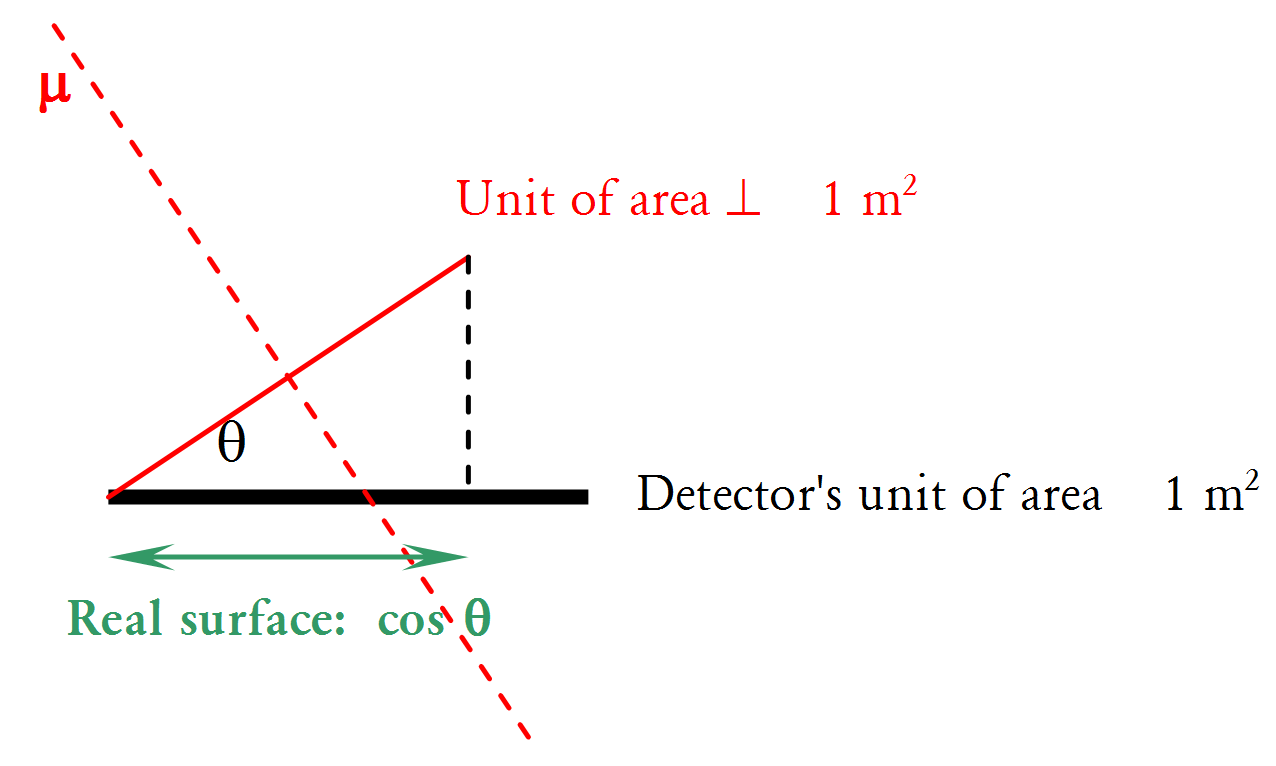
\includegraphics[width=.9\textwidth]{img/app1.png}
			\captionsetup{width=0.8\textwidth}\caption
				[Schematic view of the incident particle path.]
				{Schematic view of the incident particle path.}\label{fig:app1}
		\ec
	\efi
	\end{minipage}\captionsetup{width=0.8\textwidth}



	\bc $dA = dS \cos\theta$ \ec

\textit{i.e.} solve the following integral:

	\be
		\begin{split}
			I &= \int J \,dA \\
			  &= \int_0^S \left| j(\theta,\varphi) \right| \,dS \,\cos\theta \\
			  &= \int_0^S\int_0^{2\pi}\int_0^{\pi/2} J_0 \,\cos^3\theta \sin\theta \,d\theta \,d\varphi \,dS \\
			  &= J_0 \,2\pi S \int_0^{\pi/2} \cos^3\theta \sin\theta \,d\theta
		\end{split}
	\ee

The last integral, which only has dependence on $\theta$, is easily solved by:

	\be
		\begin{split}
			\int_0^{\pi/2} \cos^3\theta \sin\theta \,d\theta &= 
			\int_0^{\pi/2} \left[ -\frac{1}{4}\frac{d(\cos^4\theta)}{d\theta}\right] d\theta \\
			&= \frac{1}{4}\int_0^1 d(\cos^4\theta) \\
			&= \frac{1}{4} 
		\end{split}
	\ee

thus obtaining:

	\be I = J_0 \,\frac{\pi}{2}S\frac{part.}{s} = \frac{N}{t}\ee

which is simply the total intensity of particles per unit time reaching the scintillator detector with rectangular geometry and surface $S$, and equals the number of counts per unit time to be registered in it (after noise substraction).

For the soft component we can assume to a first approximation that the distribution is equal to that of the hard component.
